\documentclass{standalone}
\usepackage{tikz}
\usepackage{tikz-qtree}
\usepackage[makeroom]{cancel}
\usetikzlibrary{fit}


\begin{document} 
	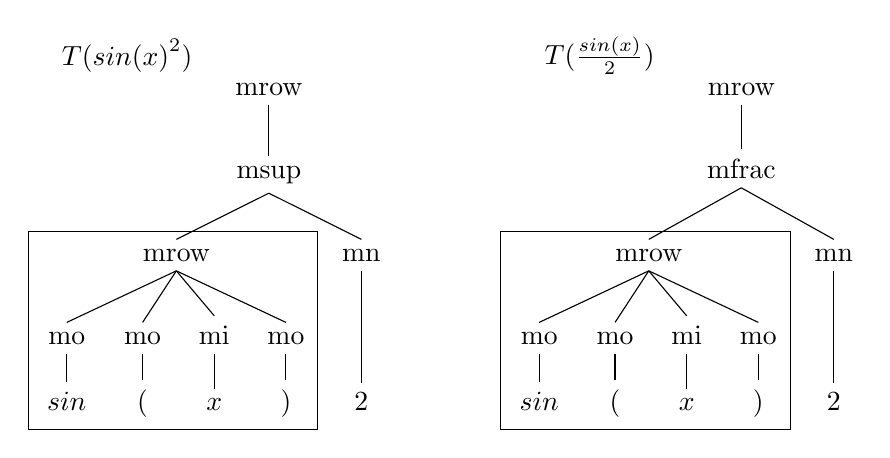
\begin{tikzpicture}[sibling distance=7pt]

		\tikzset{frontier/.style={distance from root=9.5\baselineskip}}
	    \node (x) at (-1.8,0.5) {$T({sin(x)}^2)$};
	    \Tree [.mrow
	    		[.msup
		            [.mrow
		                [.mo \node(sin){$sin$}; ]
		                [.mo $($ ]
		                [.mi $x$ ]
		                [.mo $)$ ] 
		            ] 
		            [.mn $2$ ]
		        ]
	          ]
	    \node (x) at (0.25,-2.1) {\phantom{X}};
	    \node[draw,fit=(sin)(x)]{};
	    

	    \begin{scope}[xshift=6.0cm]
	    \node (y) at (-1.8,0.5) {$T(\frac{sin(x)}{2})$} ;
	    \Tree [.mrow
	    		[.mfrac
		            [.mrow
		                [.mo \node(sin){$sin$}; ]
		                [.mo $($ ]
		                [.mi $x$ ]
		                [.mo $)$ ] 
		            ] 
		            [.mn $2$ ]
		        ]
	          ]
	    \node (y) at (0.25,-2.1) {\phantom{X}};
	    \node[draw,fit=(sin)(y)]{};
	    \end{scope}


	\end{tikzpicture}
\end{document} 